\newpage
\section{Implementations}
\subsection{NTL et FLINT}
We first sought to measure the performance given to us by existing software. Thus, we can then try to improve them or at least get closer to their performance.
Our work concentrates on polynomials. As such the classes used in both the FLINT and the NTL library relate to polynomial operations.
\subsubsection{NTL}

We started out by familiarizing ourselves with C++ and and the NTL library.
After implementing different time measurement functions we found these results for different degrees of polynomials on different operations but with a fixed set of bits at 60 (the number will be on 60 bits) and generating a polynome with FFTInit (which is way faster then GenPrime\_long which generates a polynome by using different FFT techniques).
The commands we used looked like this 
\begin{lstlisting}[language=bash]
./graph <choice of implementation> <choice of operation> 
<degree of polynomial> <number of bits> <file to save results (TODO)>
<choice of implementation> can either be
        - 0 : using a FFT generated polynomial
        - 1 : using a bits generated polynomial
<choice of operation> can be:
        - 0 : addition
        - 1 : multiplication
        - 2 : GCD
        - 3 : division  (divided by 2 by default (TODO))
        - 4 : XGCD 
For example, you could try ./ntl 0 1 1000 60
Polynome generated with FFT
./ntl 0 1 10000000 60
\end{lstlisting}

(A CHANGER : serait-il possible d'avoir les informations sur l'ordinateur que vous avez utilise ? (notamment avec la commande lshw ou uname -a par exemple))
Also, these operations were run on a macOS Monterey with a Apple M1 chip and 16GB of RAM. The computer was plugged in during these computations.
Running the command 
\begin{lstlisting}[language=bash]
uname -a 
\end{lstlisting}
gives us:
\begin{lstlisting}[language=bash]
Darwin elinas-macbook-air.home 21.6.0 Darwin Kernel Version 21.6.0: Sat Jun 18 17:05:47 PDT 2022; root:xnu-8020.140.41~1/RELEASE_ARM64_T8101 arm64
\end{lstlisting}
FLINT and NTL are two well-known libraries for performing arithmetic operations on integers and polynomials over finite fields. Both libraries provide efficient implementations of basic arithmetic operations such as addition, subtraction, multiplication, and division. In addition to these operations, both libraries also provide algorithms for computing the greatest common divisor (GCD) and extended GCD (XGCD) of two integers or polynomials.
\newline 
In this comparison, we will focus on the performance of FLINT and NTL for division, multiplication, GCD and XGCD operations. 
\newline 
We will first provide an overview of FLINT and NTL and their features. Then, we will discuss the algorithms used by both libraries, present our findings for division, multiplication GCD and XGCD, and compare their performance. 
\newline
\newline We get these results for polynomial multiplication and division:
\begin{figure}[H]
    \centering
    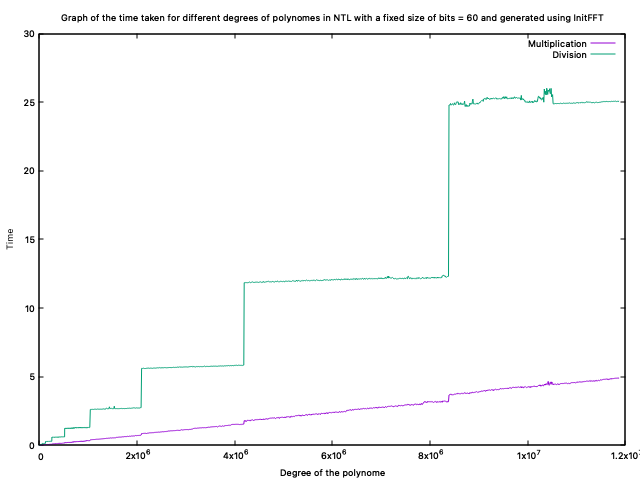
\includegraphics[width=0.85\textwidth]{figures/ntl_mult_div.png}
    \label{fig2}
    \caption{Multiplication and division in NTL}
\end{figure}
NTL uses the Karatsuba algorithm for small polynomials and the Fast Fourier Transform (FFT) or NTT for larger polynomials. The complexity for polynomial multiplication using these algorithms is:
\begin{itemize}
    \item Karatsuba: $O(n^{1.585})$, where $n$ is the degree of the polynomials
    \item FFT-based algorithms: $O(n\log(n))$
    \item NTT-based algorithms: $O(n\log(n))$
\end{itemize}
For the polynomial division, NTL uses the classical polynomial division algorithm, which has a complexity of:
\begin{itemize}
    \item Classical division: $O(n^2)$, where $n$ is the degree of the divisor polynomial
\end{itemize}

For the GCD and the XGCD we get the graphs :
\begin{figure}[H]
    \centering
    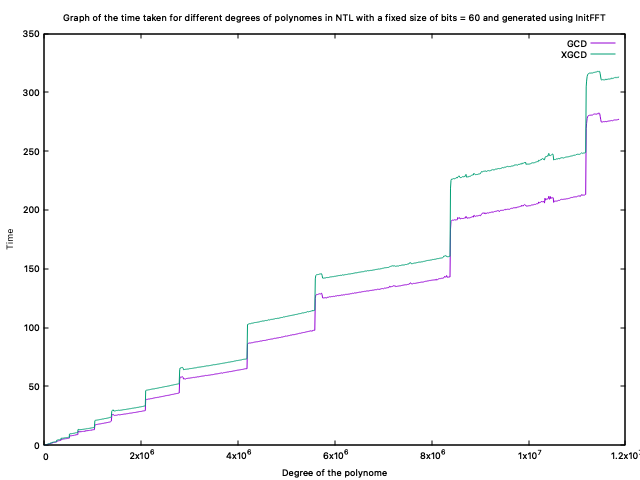
\includegraphics[width=0.85\textwidth]{figures/ntl_gcd_xgcd.png}
    \label{fig2}
    \caption{GCD and XGCD (a*u + b*v = p format) in NTL}
\end{figure}

For polynomial GCD and XGCD computations, NTL uses the Euclidean algorithm. The complexity of this algorithm is:
\begin{itemize}
    \item algorithm NTL uses for computing the GCD of two integers is the binary GCD algorithm (also known as the Stein's algorithm). The binary GCD algorithm has a worst-case time complexity of O($log (n)^2$), where n is the maximum number of bits in the input integers.
    \item For computing the XGCD of two integers, NTL uses the extended binary GCD algorithm, which is a variant of the binary GCD algorithm. The extended binary GCD algorithm has a worst-case time complexity of O($log (n)^2$), where n is the maximum number of bits in the input integers.
\end{itemize}
\subsubsection{FLINT}

Then we wanted to measure the results for another popular library for number theory FLINT. 
To get better and more representative results, we separated the XGCD and the GCD from the multiplication and the division as those operations were closer to each other in terms of the time they were taking.

For the multiplication and the division we get:
\begin{figure}[H]
    \centering
    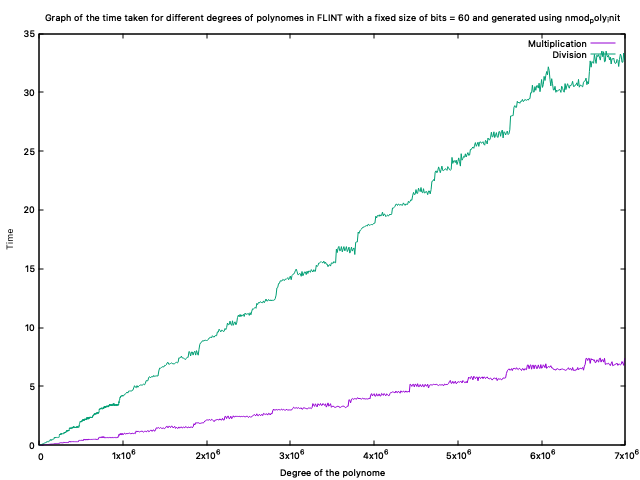
\includegraphics[width=0.85\textwidth]{figures/flint_mult_div.png}
    \label{fig2}
    \caption{Multiplication and division in FLINT}
\end{figure}
For polynomial multiplication, FLINT uses a combination of algorithms, such as the schoolbook method for small polynomials, Karatsuba's algorithm for medium-sized polynomials, and the Fast Fourier Transform (FFT) or NTT for large polynomials. The complexity of these algorithms is:
\begin{itemize}
    \item Schoolbook method: $O(n^2)$, where $n$ is the degree of the input polynomials
    \item Karatsuba's algorithm: $O(n^{1.585})$, where $n$ is the degree of the input polynomials
    \item FFT-based algorithms: $O(n \log(n))$, where $n$ is the degree of the input polynomials
    \item NTT-based algorithms: $O(n \log(n))$, where $n$ is the degree of the input polynomials
\end{itemize}
For polynomial division, FLINT uses the classical polynomial division algorithm, which has a complexity of:
\begin{itemize}
    \item Classical division: $O(n^2)$, where $n$ is the degree of the divisor polynomial
\end{itemize}

And for the GCD and the XGCD we get the graphs :
\begin{figure}[H]
    \centering
    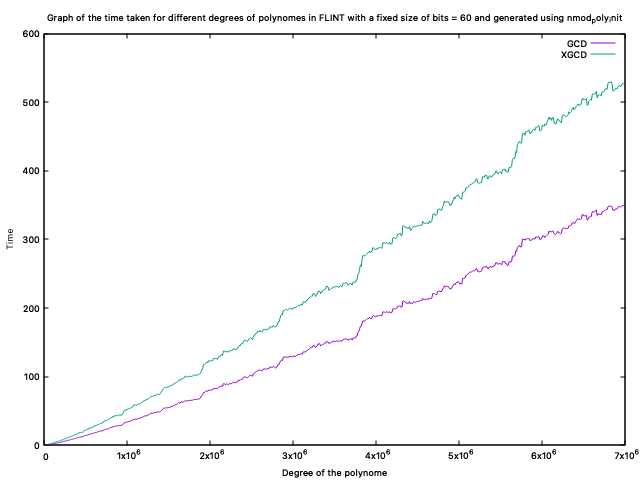
\includegraphics[width=0.85\textwidth]{figures/flint_gcd_xgcd.png}
    \label{fig2}
    \caption{GCD and XGCD (a*u + b*v = p format) in FLINT}
\end{figure}
For polynomial GCD and XGCD computations, FLINT uses various algorithms depending on the input size, such as the Euclidean algorithm for small input polynomials and the half-GCD algorithm for larger input polynomials. The complexity of these algorithms is:
\begin{itemize}
    \item Euclidean algorithm: $O(n^2)$, where $n$ is the degree of the input polynomials
    \item Half-GCD algorithm: $O(n \log^2(n))$, where $n$ is the degree of the input polynomials
\end{itemize}

\qquad As such those are the results we want to approximate using our algorithm.
\subsubsection{Comparaison between FLINT and NTL}
\newline NTL (Number Theory Library) and FLINT (Fast Library for Number Theory) are two widely-used libraries for implementing efficient algorithms for number theory computations. Both libraries provide implementations of algorithms for basic number theory tasks such as prime generation, factoring, and computing greatest common divisors (GCDs) and extended GCDs. In this comparison, we will focus specifically on the performance of these libraries for computing multiplication, division GCDs and extended GCDs.
\newline
\newline In this comparison, we will focus on the performance of FLINT and NTL for division and multiplication operations. Division and multiplication are fundamental arithmetic operations and are used extensively in many computational tasks. Therefore, the performance of these operations is of great importance in many applications, especially in cryptography and coding theory.
\newline
\begin{itemize}
\item Division and multiplication :
\end{itemize}
While comparing the two graphs of NTL and FLINT we can see that:
\newline
- For multiplication it's very efficient for both algorithm but we see that NTL is slightly faster than FLINT
\newline
- Concerning division NTL they're still efficient as algorithms but NTL is faster than FLINT for example to compute division of a polynomial of degree $6x10^6$ it only takes about $12s$ for NTL while is takes more than $30s$ for FLINT.
\newline
\begin{itemize}
\item GCD and XGCD :
\end{itemize}
The GCD is a fundamental operation in number theory and has numerous applications in cryptography, coding theory, and other areas. The extended GCD is a more general algorithm that computes not only the GCD, but also the coefficients of a linear combination of the input numbers that equals their GCD. Therefore, the extended GCD is a powerful tool for solving Diophantine equations and other problems in number theory.
\newline
\newline Next, we will examine the performance of the GCD and extended GCD algorithms in NTL and FLINT, and compare their speed and efficiency.
\newline When we see the two graphs of NTL and FLINT for computing The GCD and XGCD we can see that :
\newline - For the GCD, NTL takes $130s$ for computing the GCD of a polynomial of degree $6x10^6$ while FLINT over $320s$ for a polynomial of the same degree, we can also see that the FLINT graph grows faster than NTL's.
\newline - For the XGCD, NTL takes $150$ for computing the GCD of a polynomial of degree $6x10^6$ while FLINT over $500s$ for a polynomial of the same degree, we can also see that the FLINT graph grows faster than NTL's.
\newline So we can say that NTL is faster than FLINT for computing GCD and XGCD for polynomials of high degrees
